\documentclass[11pt,twocolumn,oneside,openany,headings=optiontotoc,11pt,numbers=noenddot]{article}

\usepackage[a4paper]{geometry}
\usepackage[utf8]{inputenc}
\usepackage[T1]{fontenc}
\usepackage{lmodern}
\usepackage[ngerman]{babel}
\usepackage{ngerman}

\usepackage[onehalfspacing]{setspace}

\usepackage{fancyhdr}
\usepackage{fancybox}

\usepackage{rotating}
\usepackage{varwidth}

%Struktogramme
\usepackage[german,curves]{struktex}

\usepackage{pdflscape}
\usepackage{changepage}
\usepackage{graphicx}
\usepackage[bottom]{footmisc}
\usepackage{transparent}
\usepackage{graphbox}
\graphicspath{
	{Pics/PDFs/}
	{Pics/JPGs/}
	{Pics/PNGs/}
}
\usepackage{caption}
\usepackage{wrapfig}
\usepackage{marginnote}
\usepackage{tabularx}
\usepackage{dashrule}
\usepackage{soulutf8}
\usepackage{hhline}
%arydshln suppresses vertical lines in table
%\usepackage{arydshln}
\usepackage{multirow}
\usepackage{enumerate}
\usepackage[hidelinks]{hyperref}
\usepackage{listings}

\usepackage[table]{xcolor}
\usepackage{array}
\usepackage{enumitem,amssymb,amsmath}
\usepackage{interval}
\usepackage{cancel}
\usepackage{stmaryrd}
\usepackage{wasysym}
\usepackage{polynom}
\usepackage{diagbox}
\usepackage{dashrule}
\usepackage{framed}
\usepackage{mdframed}
\usepackage{karnaugh-map}
\usepackage{pdfpages}

\usepackage{blindtext}

\usepackage{eso-pic}

\usepackage{amssymb}
\usepackage{eurosym}

\usepackage[pages=some]{background}
\pagestyle{headings}
\renewcommand{\headrulewidth}{0.2pt}
\renewcommand{\footrulewidth}{0.2pt}
\newcommand*{\underdownarrow}[2]{\ensuremath{\underset{\overset{\Big\downarrow}{#2}}{#1}}}
\setlength{\fboxsep}{5pt}
\newcommand{\explainBelow}[3]{\underbrace{#1}_{\parbox{\widthof{#3}}{\footnotesize\raggedright #2}}}
\newcommand{\explainAbove}[3]{\overbrace{#1}^{\parbox{\widthof{#3}}{\footnotesize\raggedright #2}}}
\newcommand\footnoteref[1]{\protected@xdef\@thefnmark{\ref{#1}}\@footnotemark}


% Codestyle defined
\definecolor{codegreen}{rgb}{0,0.6,0}
\definecolor{codegray}{rgb}{0.5,0.5,0.5}
\definecolor{codepurple}{rgb}{0.58,0,0.82}
\definecolor{backcolour}{rgb}{0.95,0.95,0.92}
\definecolor{deepgreen}{rgb}{0,0.5,0}
\definecolor{darkblue}{rgb}{0,0,0.65}
\definecolor{mauve}{rgb}{0.40, 0.19,0.28}
\colorlet{exceptioncolour}{yellow!50!red}
\colorlet{commandcolour}{blue!60!black}
\colorlet{numpycolour}{blue!60!green}
\colorlet{specmethodcolour}{violet}

%Neue Spaltendefinition
\newcolumntype{L}[1]{>{\raggedright\let\newline\\\arraybackslash\hspace{0pt}}m{#1}}
\newcolumntype{M}{>{\centering\arraybackslash}X}
\newcommand{\cmnt}[1]{\ignorespaces}
%Textausrichtung ändern
\newcommand\tabrotate[1]{\rotatebox{90}{\raggedright#1\hspace{\tabcolsep}}}

%Intervall-Konfig
\intervalconfig {
	soft open fences
}

%Bash
\lstdefinestyle{BashInputStyle}{
	language=bash,
	basicstyle=\small\sffamily,
	backgroundcolor=\color{backcolour},
	columns=fullflexible,
	backgroundcolor=\color{backcolour},
	breaklines=true,
}
%Java
\lstdefinestyle{JavaInputStyle}{
	language=Java,
	backgroundcolor=\color{backcolour},
	aboveskip=1mm,
	belowskip=1mm,
	showstringspaces=false,
	columns=flexible,
	basicstyle={\footnotesize\ttfamily},
	numberstyle={\tiny},
	numbers=none,
	keywordstyle=\color{purple},,
	commentstyle=\color{deepgreen},
	stringstyle=\color{blue},
	emph={out},
	emphstyle=\color{darkblue},
	emph={[2]rand},
	emphstyle=[2]\color{specmethodcolour},
	breaklines=true,
	breakatwhitespace=true,
	tabsize=2,
}
%Python
\lstdefinestyle{PythonInputStyle}{
	language=Python,
	alsoletter={1234567890},
	aboveskip=1ex,
	basicstyle=\footnotesize,
	breaklines=true,
	breakatwhitespace= true,
	backgroundcolor=\color{backcolour},
	commentstyle=\color{red},
	otherkeywords={\ , \}, \{, \&,\|},
	emph={and,break,class,continue,def,yield,del,elif,else,%
		except,exec,finally,for,from,global,if,import,in,%
		lambda,not,or,pass,print,raise,return,try,while,assert},
	emphstyle=\color{exceptioncolour},
	emph={[2]True,False,None,min},
	emphstyle=[2]\color{specmethodcolour},
	emph={[3]object,type,isinstance,copy,deepcopy,zip,enumerate,reversed,list,len,dict,tuple,xrange,append,execfile,real,imag,reduce,str,repr},
	emphstyle=[3]\color{commandcolour},
	emph={[4]ode, fsolve, sqrt, exp, sin, cos, arccos, pi,  array, norm, solve, dot, arange, , isscalar, max, sum, flatten, shape, reshape, find, any, all, abs, plot, linspace, legend, quad, polyval,polyfit, hstack, concatenate,vstack,column_stack,empty,zeros,ones,rand,vander,grid,pcolor,eig,eigs,eigvals,svd,qr,tan,det,logspace,roll,mean,cumsum,cumprod,diff,vectorize,lstsq,cla,eye,xlabel,ylabel,squeeze},
	emphstyle=[4]\color{numpycolour},
	emph={[5]__init__,__add__,__mul__,__div__,__sub__,__call__,__getitem__,__setitem__,__eq__,__ne__,__nonzero__,__rmul__,__radd__,__repr__,__str__,__get__,__truediv__,__pow__,__name__,__future__,__all__},
	emphstyle=[5]\color{specmethodcolour},
	emph={[6]assert,range,yield},
	emphstyle=[6]\color{specmethodcolour}\bfseries,
	emph={[7]Exception,NameError,IndexError,SyntaxError,TypeError,ValueError,OverflowError,ZeroDivisionError,KeyboardInterrupt},
	emphstyle=[7]\color{specmethodcolour}\bfseries,
	emph={[8]taster,send,sendMail,capture,check,noMsg,go,move,switch,humTem,ventilate,buzz},
	emphstyle=[8]\color{blue},
	keywordstyle=\color{blue}\bfseries,
	rulecolor=\color{black!40},
	showstringspaces=false,
	stringstyle=\color{deepgreen}
}

\lstset{literate=%
	{Ö}{{\"O}}1
	{Ä}{{\"A}}1
	{Ü}{{\"U}}1
	{ß}{{\ss}}1
	{ü}{{\"u}}1
	{ä}{{\"a}}1
	{ö}{{\"o}}1
}

% Neue Klassenarbeits-Umgebung
\newenvironment{worksheet}[3]
% Begin-Bereich
{
	\newpage
	\sffamily
	\setcounter{page}{1}
	\ClearShipoutPicture
	\AddToShipoutPicture{
		\put(55,761){{
				\mbox{\parbox{385\unitlength}{\tiny \color{codegray}BBS I Mainz, #1 \newline #2
						\newline #3
					}
				}
			}
		}
		\put(455,761){{
				\mbox{\hspace{0.3cm}
\includegraphics[width=0.2\textwidth]{../../logo.pdf}}
			}
		}
	}
}
% End-Bereich
{
	\clearpage
	\ClearShipoutPicture
}

\setlength{\columnsep}{3em}
\setlength{\columnseprule}{0.5pt}

\geometry{left=1.50cm,right=1.50cm,top=3.00cm,bottom=1.00cm,includeheadfoot}
\pagenumbering{gobble}
\pagestyle{empty}

\begin{document}
	\begin{worksheet}{BBS I, Höhere Berufsfachschule IT-Systeme}{Grundstufe - Mathematik}{Lernabschnitt 4: Differenzialrechnung - Kurvendiskussion - Wendestellen}
		\setcounter{section}{7}
		\setcounter{subsection}{4}
		\subsection{Wendestellen}
		Skizzieren wir den Graphen einer ganzrationalen Funktion, so kann dieser links- aber auch eine rechtsgekrümmt verlaufen. Wenn wir ihn zeichnen, zeichnen wir in diesem Abschnitt eine nach oben (linksgekrümmt) oder nach unten (rechtsgekrümmt) geöffnete Parabel. Zwischen einer Links- und einer Rechtskrümmung ändert der Graph seine \textbf{Krümmungsrichtung}. Der Punkt, an dem dies geschieht, bezeichnet man als \textbf{Wendepunkt}.
		\subsection*{Rechnerische Bestimmung der Wendestellen}
		Wir haben bereits herausgefunden, dass man mit der ersten Ableitung \(f'(x)\) die Extremstellen\footnote{Hoch- bzw. Tiefpunkt.} der Funktion bestimmen kann.\\
		Betrachten wir uns die Graphen von \(f(x)\), kann man vermuten, dass die Wendestelle zwischen zwei Extrempunkten (zwischen Hoch- und Tiefpunkt bzw. zwischen Tief- und Hochpunkt) liegt.\\
		Schauen wir uns den Ableitungsgraphen \(f'(x)\) an, sehen wir, dass zwischen dessen Nullstellen wieder ein Extrempunkt liegt.\\
		\par\noindent
		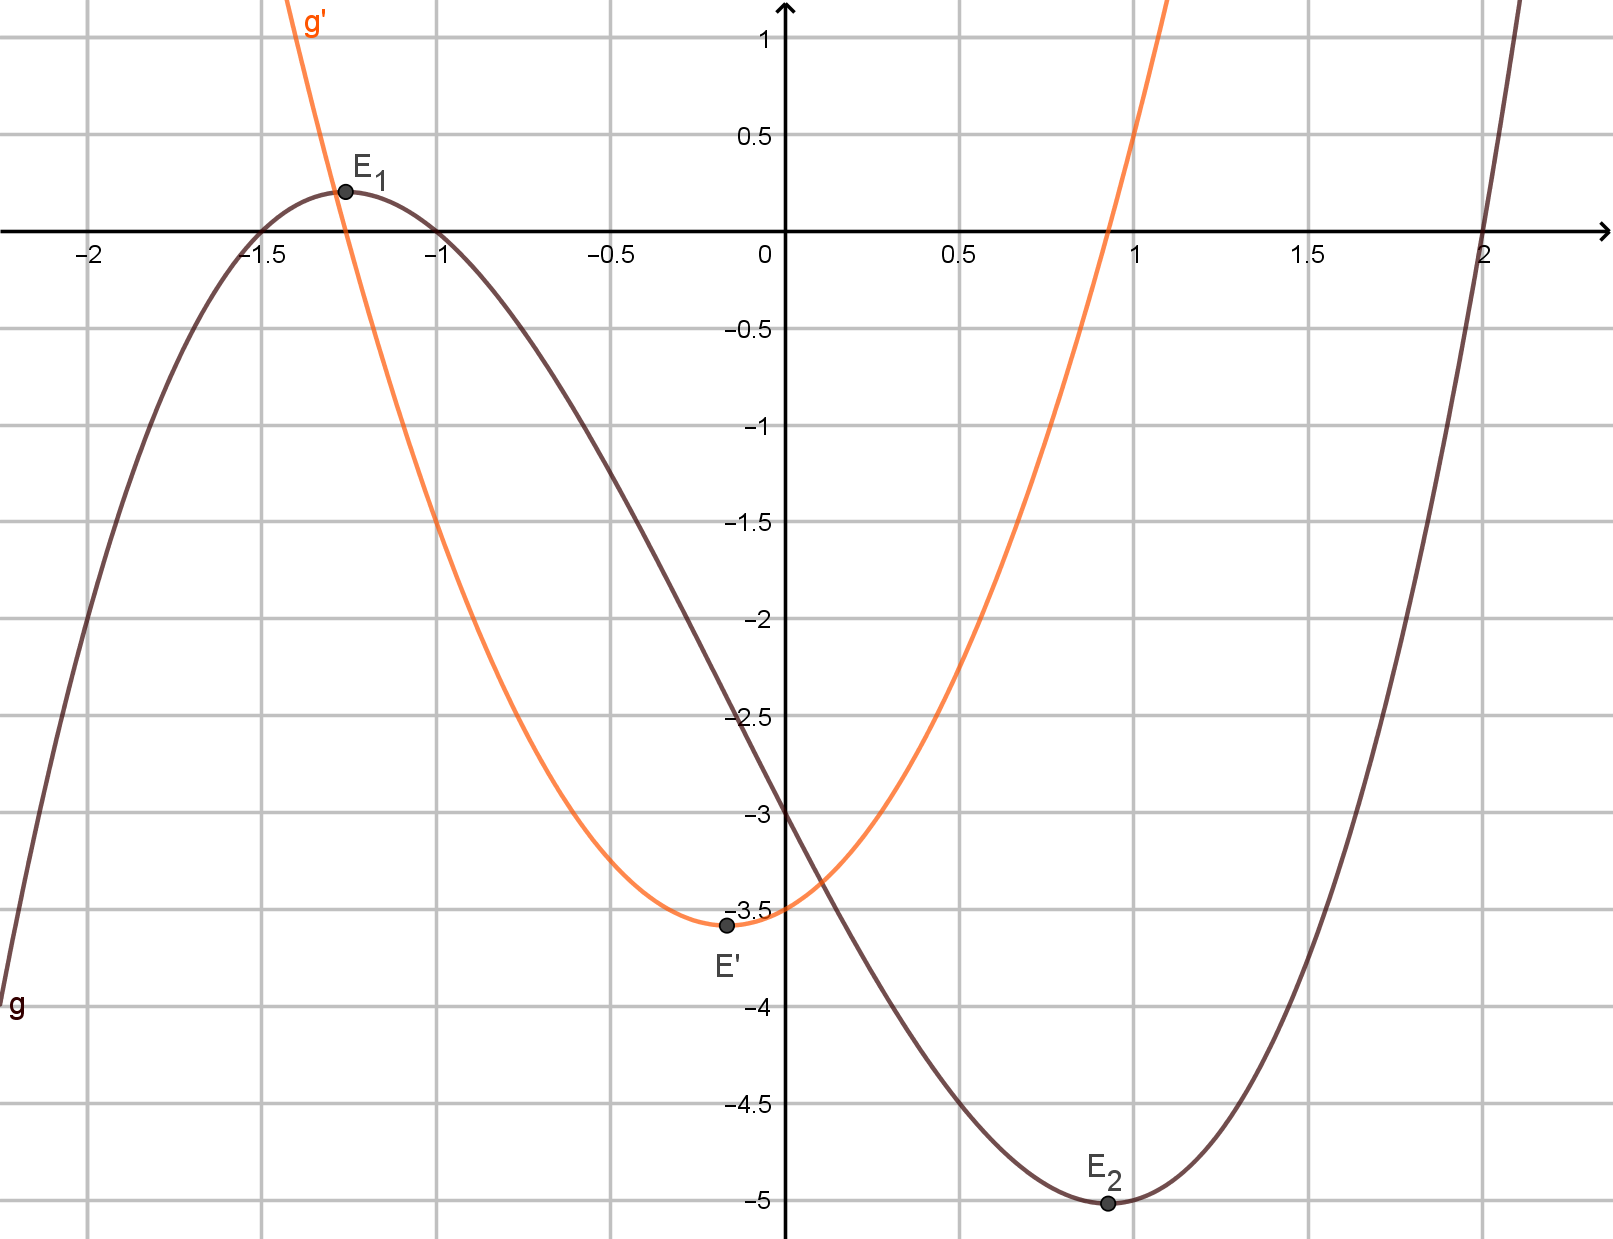
\includegraphics[width=0.48\textwidth]{../99_Bilder/045_WS_Einf.png}\\
		Um also diese Stelle bestimmen zu können, müssen wir die Extremstelle der ersten Ableitung berechnen.\\
		Hierfür bestimmen wir die Nullstellen der Ableitung der ersten Ableitung - also die Nullstellen der zweiten Ableitung \(f''(x)\).\\
		Haben wir diese berechnet, müssen wir mit der dritten Ableitung prüfen, ob es sich auch wirklich um eine Wendestelle handelt. Dies ist nur der Fall, wenn \(f''(x_W)\) an der Stelle \(x_W\) das Vorzeichen wechselt.\\
		\par\noindent
		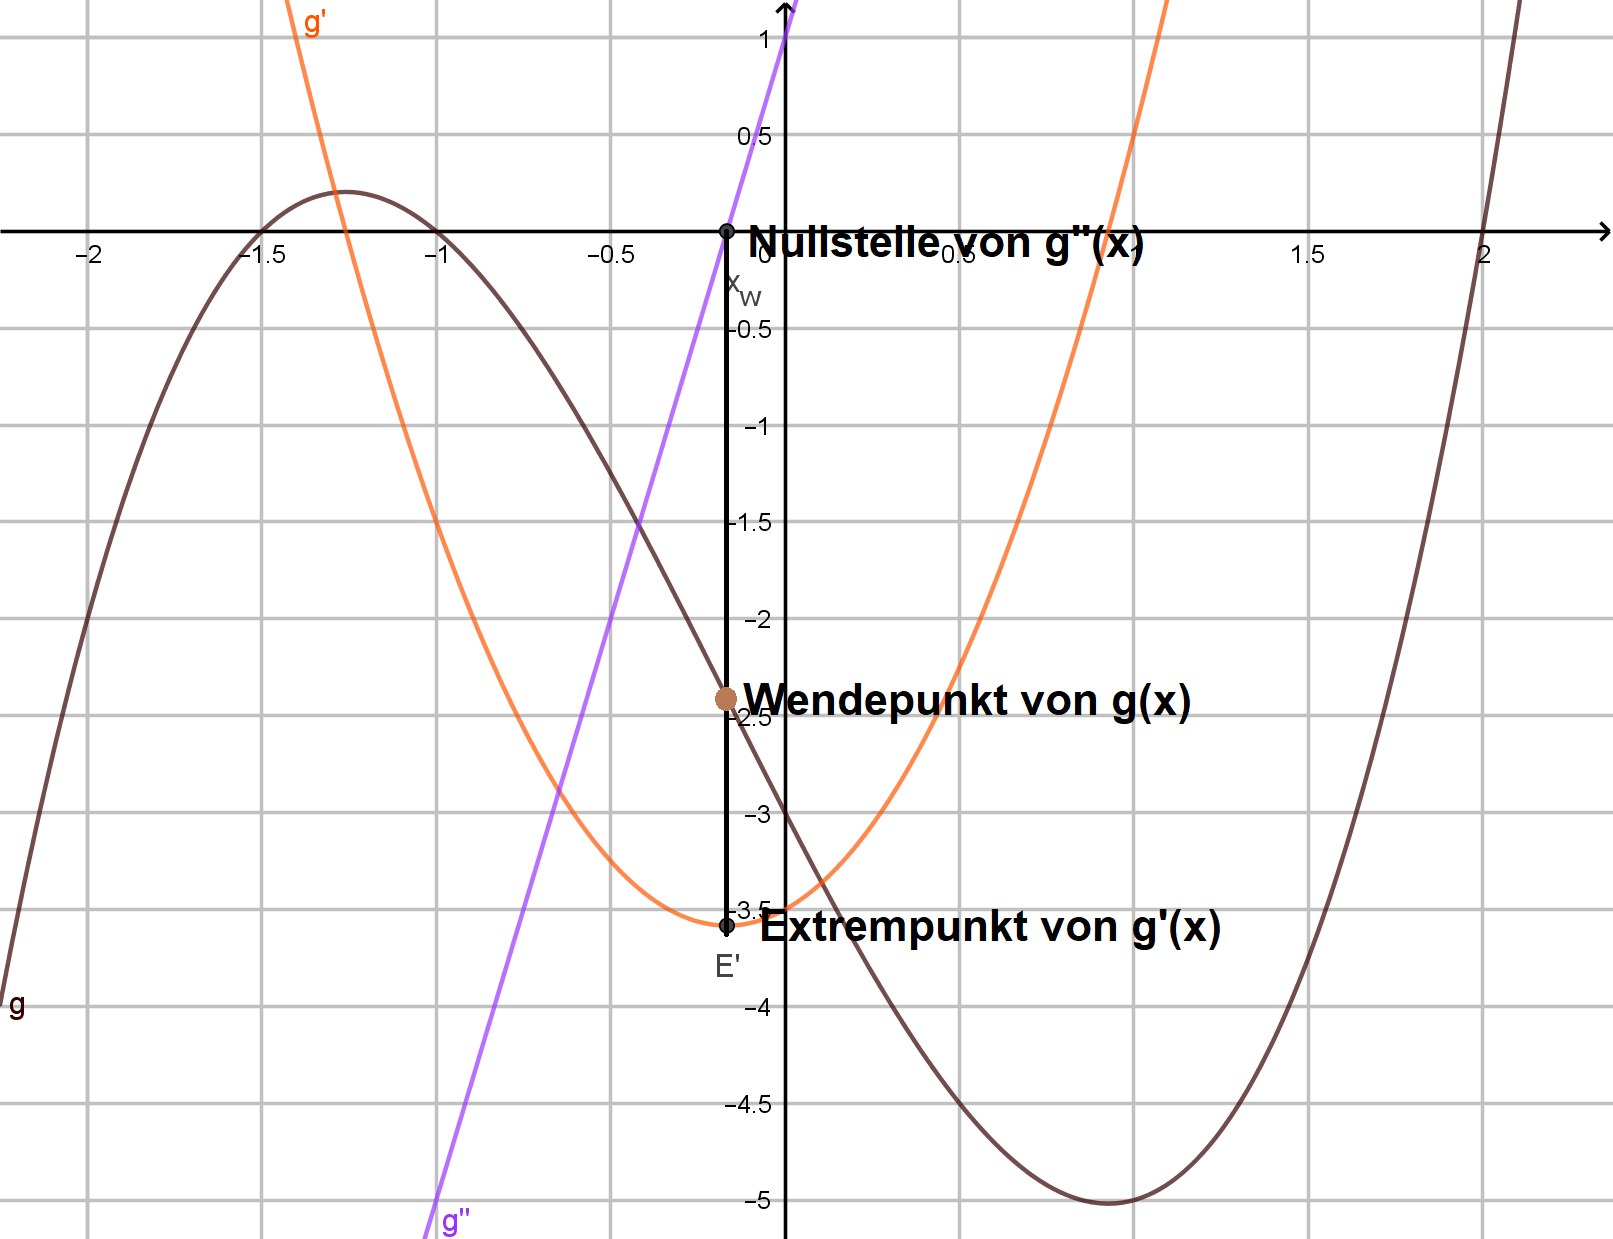
\includegraphics[width=0.48\textwidth]{../99_Bilder/045_WS_VZW.png}
		\begin{framed}
			\(x_W\) ist eine Wendestelle von \(f(x)\), wenn
			\begin{itemize}
				\item[-] \textbf{notwendige Bedingung:}\\
				\(f''(x_W) = 0\)
			\end{itemize}
			und
			\begin{itemize}
				\item[-] \textbf{hinreichende Bedingung:}\\
				\(f''(x_W)\) hat Vorzeichenwechsel
				\begin{itemize}
					\item von \glqq{}+\grqq{} nach \glqq{}-\grqq{}\\
					\(x_W\) ist Wendestelle mit L-R-Übergang
					\item \glqq{}-\grqq{} nach \glqq{}+\grqq{}\\
					\(x_W\) ist Wendestelle mit R-L-Übergang
				\end{itemize}
				oder\\
				\(f'''(x_W)\neq 0\)\\
			\end{itemize}
		\end{framed}
		\newpage
		\noindent
		\textbf{Beispiel:} \(f(x) = x^3 + 0,5x^2 -3,5x -3\)\\
		Im vergangenen Abschnitt haben wir bereits die erste und zweite Ableitung bestimmt.\\
		\(f'(x) = 3x^2 + x -3,5\)\\
		\(f''(x) = 6x + 1\)\\
		\par\noindent
		Um nun die Nullstellen der zweiten Ableitung zu bestimmen, setzen wir diese gleich Null (0) und formen anschließend nach \(x\) um.
		\begin{align*}
			0 & = 6x +1 & |-1\\
			-1 & = 6x & |:6\\
			-\frac{1}{6} & = x
		\end{align*}
		Wir wissen nun, \(x_W = -\frac{1}{6}\) ist eine mögliche Wendestelle von \(f(x)\). Um dies zu verifizieren, haben wir zwei Möglichkeiten.\\
		\par\noindent
		Entweder wir untersuchen, ob \(f''(x)\) bei \(x_W\) einen Vorzeichenwechsel hat. Hierfür bestimmen wir den Funktionswert für ein \(x_1 < x_w < x_2\).
		\begin{tabbing}
			\(x_1 = -1\) ~~~~~~~~~~~~~~~~~~~~~~~~~~ \= \(x_2 = 0\)\\
			\(f''(-1) = 6\cdot(-1) + 1\) \> \(f''(0) = 6\cdot{}0 + 1\)\\
			\( = -5\) \> \(= 1\)
		\end{tabbing}
		Wir sehen, \(f''(x)\) hat bei \(x_w\) einen Vorzeichenwechsel. Da wir von \glqq{}-\grqq{} nach \glqq{}+\grqq{} wechseln, handelt es sich um eine Wendestelle mit R-L-Übergang.\\
		\rule{0.48\textwidth}{0.1pt}\\
		\par\noindent
		Alternativ können wir auch mit der dritten Ableitung \(f'''(x)\) arbeiten.\\
		\(f'''(x) = 6\), somit ist \(f'''(x_W) = 6 > 0\) und daher eine Wendestelle mit R-L-Übergang.\\
		\color{red}{\underline{Vorsicht!}}\normalcolor{} Die Prüfung über die dritte Ableitung ist nicht sicher.\\
		Eine x-Stelle \(x_W\) kann auch Wendestelle sein, obwohl \(f'''(x_W) = 0\).
		\newpage
		\subsection{Sattelstelle}
		Nun kann es passieren, dass wir eine Wendestelle berechnen, die bereits eine Extremstelle war. Das bedeutet \[f'(x_S) = 0 \wedge f''(x_s) = 0\] Eine solche Stelle nennen wir \textbf{Sattelstelle}.\\
		\par\noindent
		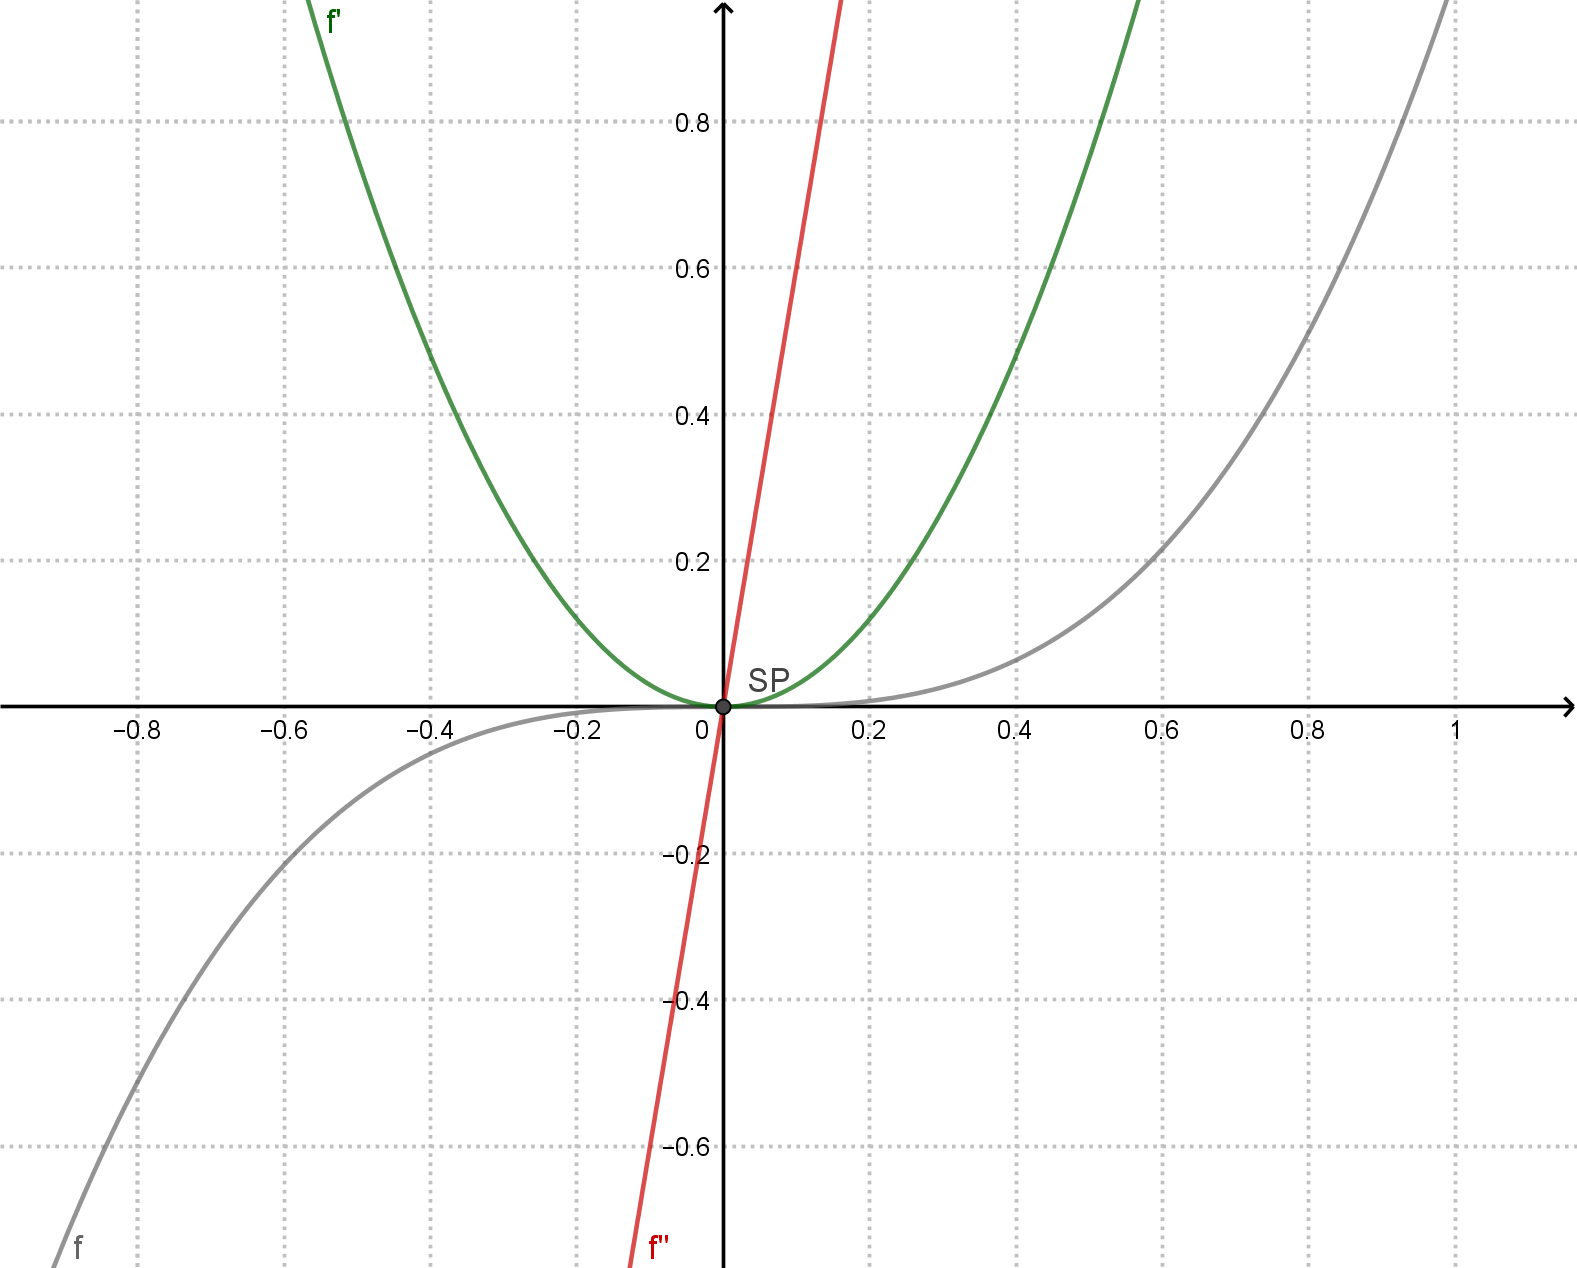
\includegraphics[width=0.48\textwidth]{../99_Bilder/045_SaS_Bsp1.png}\\
		\par\noindent
		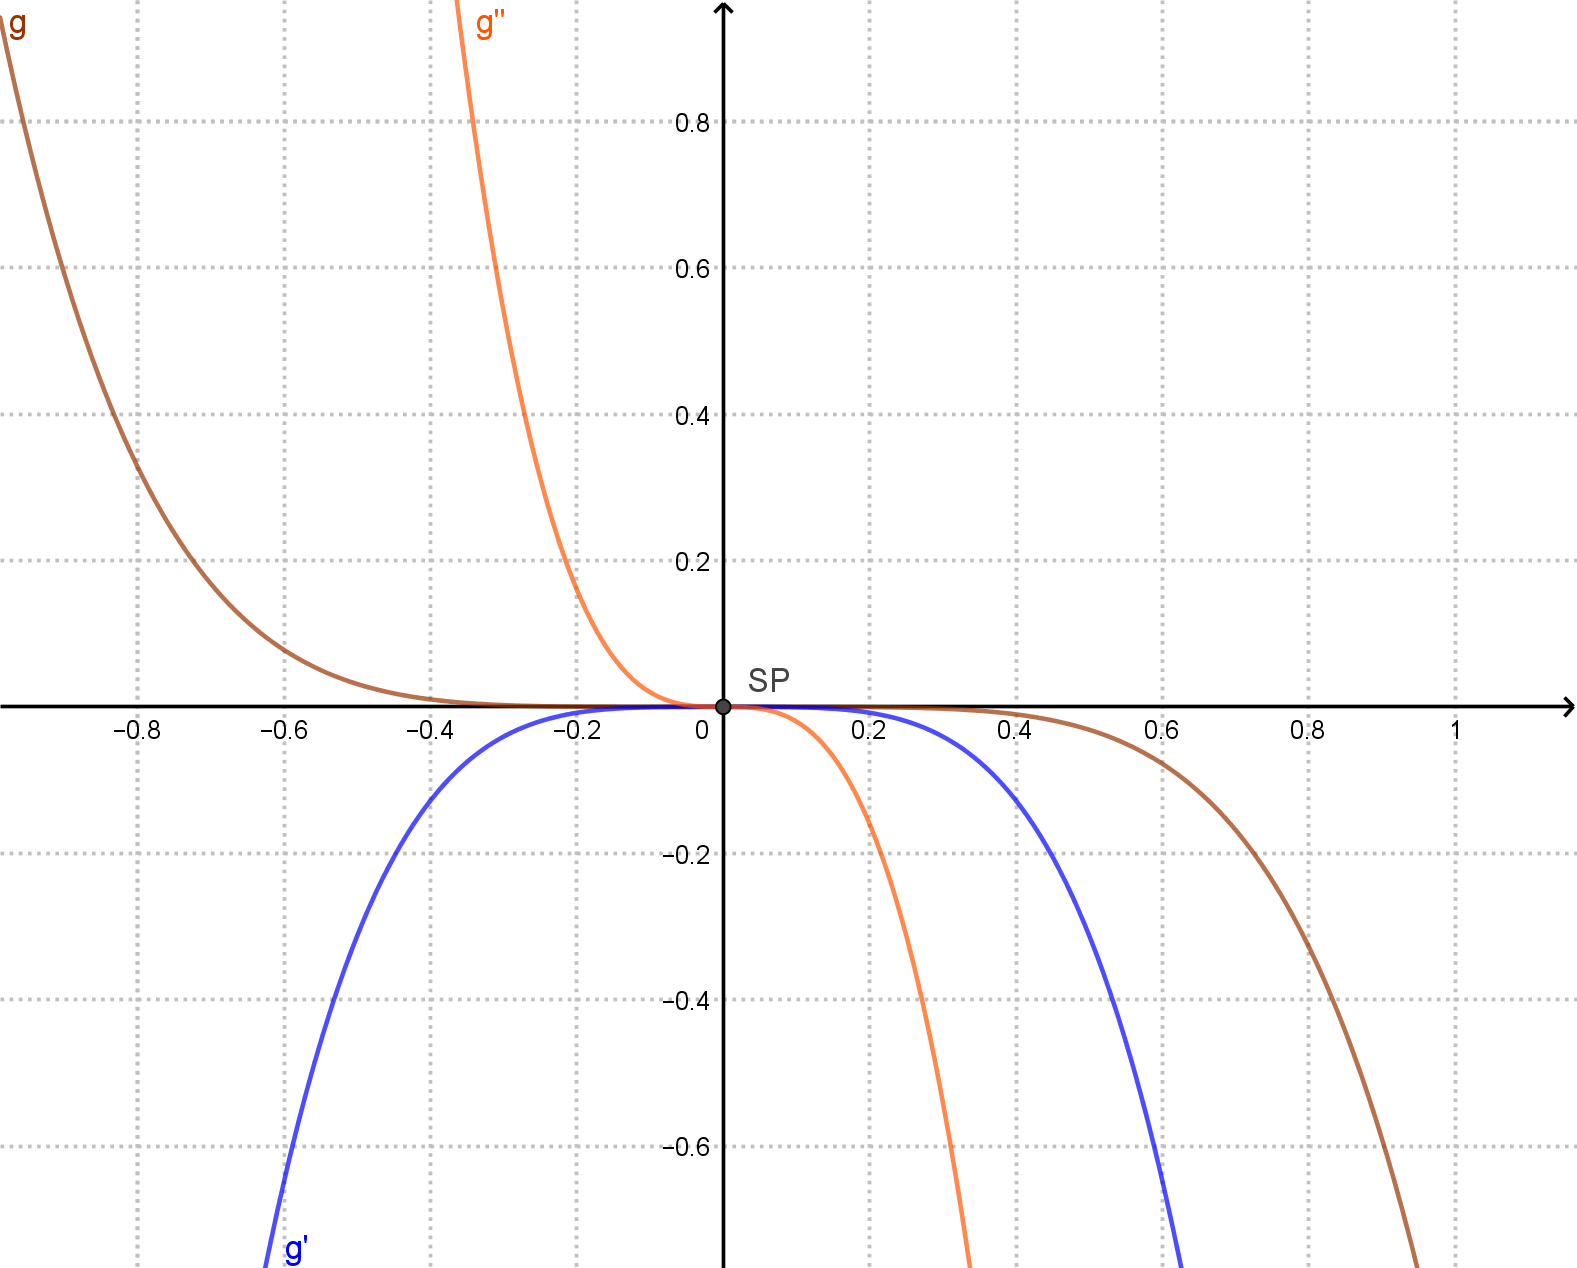
\includegraphics[width=0.48\textwidth]{../99_Bilder/045_SaS_Bsp2.png}
		\begin{framed}
			\noindent
			Ist \(\mathbf{f'(x_S) = 0}\) und \(\mathbf{f''(x_S) = 0}\), dann ist \(x_S\) weder Extrem- noch Wendestelle.\\
			\par\noindent
			In diesem Fall bezeichnen wir \(x_S\) als \textbf{Sattelstelle}.
		\end{framed}
	\end{worksheet}
\end{document}